\chapter{Quantum Thermodynamics And Canonical Typicality}
\section{Introduction}

The foundations of Statistical Mechanics remain a debatable subject. Fundamental questions have emerged form these discussions regarding the role of probabilities, entropy\footnote{Probabilities and entropy are both referred as measures of ignorance}, the relevance of time averages and ensamble averages to individual physical systems. One of the most controversial issue is the validity of the postulate of equal a priori probability, postulate that can not be proved. \\
In this chapter we are going to discuss some ideas based on typicality addresed by several authors \cite{gemmer_quantum_2004, goldstein_canonical_2006, popescu_entanglement_2006}, who have abandoned the unprovable aforementioned postulate and replace it with a new viewpoint, which is uniquely quantum, and which does not rely on any ignorance probabilities in the description of the state. Instead, is supported, and can be proved, by means of the entanglement between a physical system and it environment. 
\newline
This chapter will be divided in three parts, first we are going to introduce the postulate of equal prior probability, discussing its commencement in the foundations of statistical mechanics, the idea of an ensemble as a collection of identical systems will be introduced and the postulate of equal prior probability will be translated  to a particular version of ensemble, the microcanonical ensemble. Also a quantum version of the above-mentioned postulate will be exhibited in terms of the random phase postulate \cite{landau_statistical_2013} and the derivation of the canonical ensemble for a weakly interacting system.
\newline
The second part will be dedicated to understand entanglement and therefore we present the phenomenon of canonical typicality, where thermalisation emerges as a consequence of typicality. These ideas are taken from  \textit{S.Popescu, A. J. short and A. Winter} \cite{popescu_entanglement_2006, popescu_foundations_2005} work which we follow very closely\footnote{However ,it is important to stress that an independet work done by \textit{Goldstein et. al.} \cite{goldstein_canonical_2006} discuss a similar issues addressed by  \textit{S.Popescu et. al.} in \cite{popescu_entanglement_2006, popescu_foundations_2005}.}. Quantitative arguments will be provided and explained with its respective mathematical tools needed to comprehend the ideas in which typicality is built on.
\newline
To conclude, we take the results obtained in the second part to present in the third part an approach studied by \textit{Linden et. al.} \cite{linden_quantum_2009} in which rather than a kinematic insight, they address the dynamical aspects of thermalisation, explaining a mechanism in which systems far from equilibrium would reach a generic state\footnote{Here a generic state has to be understood as a typical state, meaning the one that corresponds to its canonical state.} \cite{linden_quantum_2009}. Furthermore, we will suggest what would be the main subject of study in this work, an idea which intuition is built on the ideas of typicality to show why the random phase postulate could be replace with something we call super-orthogonality over partial traces, and then giving an alternative idea of how thermalisation can occur. 

\section{Postulate of Equal a Prior Probability}
Statistical physics have been historically inspired in phenomenological thermodynamics. In fact quantities such as temperature, pressure, heat and entropy emerged as concepts to describe empirical principles. And the idea of describing a system by explaining how its microscopic constituents behave but rather in effective laws, known as \textit{the law of thermodynamics\cite{uffink_handbook_2007}}\footnote{Along all this section we follow the main ideas provided in \cite{uffink_handbook_2007} which turned up to be a very interesting historical review of statistical mechanics}. A peculiar result form these studies was the \textit{the second law of thermodynamics} which  restrain the class of natural phenomena that could actually occur.
\newline
It was not until Boltzmann, Gibbs and Maxwell that statistical physics became known as a fundamental theory in the description of the physical world. However, this approach has been a subject of strong debates. Statistical physics differ from phenomenological thermodynamics by two main reasons. The first is the consideration that the behaviour of microscopic constituents could be described with classical dynamics, and the second is the introduction of probability and statistics to deduce the laws of thermodynamics.
\newline
Let us introduce the theoretical concepts, conceived at the end of the 19th century, about the description of the microscopic world\footnote{It was Maxwell who really marks the rebirth of kinetic theory. His ideas about the how in a system of great number of particles could be described taking a frequency interpretation of the probability was the base for Boltzmann's work.  }. 
\newline
Consider a mechanical system of $N$ ($N \ggg 1$) particles subject to a time-independent potential $V$. Supposing every particle conforming the system has mass $m$ and coordinates in its phase space $(\vec{q}_i,\vec{p}_i)$ we easily see that the state of the system is represented by a point in the phase space $\Gamma$ $(\vec{q},\vec{p})=(\vec{q}_{1},\ldots,\vec{q}_{N},\vec{p}_{1},\ldots,\vec{p}_{N})$, and its time evolution follows the dynamics induced by its Hamiltonian. Moreover, imposing the restriction that the energy $E$ is conserved, the evolution is confined to a set of Hamiltonians such that fulfill this restriction ($\Sigma_{E}=\left\{(\vec{q},\vec{p})\in \Gamma | H(\vec{q},\vec{p})=E\right\}$). At this moment is when probability comes to play an important role. In \cite{boltzmann_uber_1866} Boltzmann proposed to interpret the probability associated to a particular state as the relative time spent by the system in that state\footnote{ Concretely the probability of the phase point lies in an infinitesimal region of $\Sigma_E$ is given by 
\[\rho(q, p) \mathrm{d} q \mathrm{d} p=f(q, p) \delta(H(q, p)-E) \mathrm{d} q \mathrm{d} p,\]
where $dpdq$ is the Lebesgue measure of $\Gamma$ and $f$ is a suitable function.}.. This assumption relies on the hypothesis that the total time of a measurement is extremely long if compared with the intrinsic time scales of the evolution.
\newline
By Liouville's theorem, $f$ is a constant function on all the admissible trajectories on $\Sigma_{E}$. Moreover, if we assume that the trajectory of a single point in phase space fills densely $\Sigma_E$ (Ergodic hypothesis)
\begin{equation}
\rho(\vec{q},\vec{p})\propto \delta(H(\vec{q},\vec{p})-E).
\label{CH1:Liouville_equation}
\end{equation}
With this argument Boltzmann was able to prove that thermal equilibrium could be described in terms of Maxwell's distribution of velocities.
\newline
In fact in both of his works \cite{boltzmann_zur_1871}, and \cite{boltzmann_einige_1871}, Boltzmann mentioned his dissatisfaction about the Ergodic hypothesis and slowly abandoned it. It seems that he only considered it an useful assumption for his general result
\begin{quote}
For any system for which the hypothesis is true, its equilibrium state is characterized by\footnote{This equation was first derived by Boltzmann in \cite{boltzmann_uber_1866}, and this is the first occasion where probability considerations are applied to the state of the mechanical system as whole, instead of its individual particles.},
\begin{equation}
\rho_{\mathrm{mc}}\left(p | \vec{q}_{1}, \ldots, \vec{q}_{N}\right) d p=\frac{1}{\sqrt{2 m \pi}} \frac{\Gamma\left(\frac{3N}{2}\right)}{\Gamma\left(\frac{3N-1}{2}\right)} \frac{\left(E-U-\frac{p^{2}}{2 m}\right)^{(3N-2) / 2}}{(E-U)^{(3N-3) / 2}} d p,
\end{equation}
from which an analogy to the Maxwell distribution may be recovered in the limit $N \to \infty$, regardless of any details of the inter-particle interactions, or indeed whether the system represented is a gas, fluid, solid or any other thermal body.
\end{quote}

\subsection{Postulate of Equal a Priori Probability and the Microcanonical Ensemble}

Al alternative path was taken by Gibbs who made use of an alternative idea of probability in what he named as ``ensembles''. In his book \cite{gibbs_elementary_1902} Gibbs introduce the probability as a distribution function on a collection of identical systems instead of introducing the probability as an ingredient associated to the state of a single system, as Boltzmann proposed. Gibbs considered ``ensembles'' in his pioneering treatment of statistical mechanics. His ensembles were infinite sets of macroscopically identical systems, each represented  by a point in his phase space (also called \textit{microstates}) being compatible with a single macroscopic configuration (\textit{macrostate}). It is worth stressing that this approach is not interested in following the temporal evolution of a single microscopic configuration, but rather is concerned about the distribution of all the available microscopic configurations, even if the \textit{microstate} associated is entirely fictitious.
\newline
More precisely an ensemble is introduced as a probability density function on the phase space $\Gamma$, such that the average number of \textit{microstates} in a region $R$ of $\Gamma$ is given by $\int_{R}\rho(\vec{q},\vec{p}) d\vec{q}d\vec{p}$. Furthermore, the expectation value of an observable $f:\Gamma\rightarrow\mathbb{R}$ is the average of $f$ over $\Gamma$
\begin{equation}
\braket{f} = \int_{\Gamma} f((\vec{q},\vec{p})\rho(\vec{q},\vec{p})d\vec{q}d\vec{p}.
\label{CH1:Average_ensemble}
\end{equation}
In this approach we take the condition that the ensembles must be stationary\footnote{This condition reads as
\[\frac{\partial \rho_{t}}{\partial t}=\left\{H, \rho_{t}\right\} = 0\]} , to derive the microcanonical ensemble, which is the only compatible with the conservation of energy is such that
\begin{equation}
\rho_{\mathrm{\mu c}}(\vec{q},\vec{p})=\frac{1}{\left|\Sigma_{E}\right|} \delta(H(\vec{q},\vec{p})-E),
\label{CH1:Microcanonical_ensemble}
\end{equation}
with $|\Sigma_E|$ the measure of the set $\Sigma_E$.
\newline
As mentioned before Classical statistical mechanics is built on the postulate of Equal Probability.
This result can be interpreted as follows:

\begin{quote}
\textit{All microstates accessible to an isolated system are equally probable, because there is no evidence that certain microstate should be more probable than others.}
\end{quote}
Namely, when  a macroscopic system is at equilibrium, every state compatible with the constrain of the system, is equally available (likely). Which formally is translated translates into the choice of a constant density function, called the microcanonical ensemble.
\subsection{The Ergodic Hypothesis}
We have dedicated this special section discuss a little more about the ergodic hypothesis and how Boltzmann understood this to give a formal argument of why it is needed that independent of the initial distribution, it has to evolve towards a uniform distribution (equal a prior probability). To understand this argument let us introduce couple of concepts before.
\newline
The ergodicity states an equality between ensemble and time averages of observables. Each measurement of an observable $f$ at time $t_0$ takes a certain time to accomplish. In this period of time the observable $f$ samples different values so that the effectively quantity is the time average
\begin{equation}
\frac{1}{t} \int_{0}^{t} f\left(T_{s}\left(\vec{q}_{0}, \vec{p}_{0}\right)\right) \mathrm{d} s,
\end{equation}
with ($\vec{q}_{0}, \vec{p}_{0}$) is the initial microstate (at $t=0$), and $\{T_s\}_{s\in \mathbb{R}}$ is the Hamiltonian flow generated by $H$\footnote{Here $H$ is the Hamiltonian function describing the system of $N$ particles subject to a time-independet potential $V$
\[H(\vec{q}, \vec{p})=\frac{1}{2 m} \sum_{i=1}^{N} \vec{p^{2}}_{i}+V\left(\vec{q}_{1}, \ldots, \vec{q}_{N}\right).\] }. Thus we are sampling $f$  trajectories whose initial points are ($\vec{q}_0, \vec{p}_0$). Furthermore, due to the difference in scales of time between the measurement and the intrinsic time of the microscopical constituents, it is possible to consider the limit

\begin{equation}
f^{*}\left(\vec{q}_{0},\vec{p}_{0}\right)=\lim _{t \rightarrow \infty} \frac{1}{t} \int_{0}^{t} f\left(T_{s}\left(q_{0}, p_{0}\right)\right) \mathrm{d} s.
\label{CH1:Ergodicity_1}
\end{equation}
The problem about the ergodic hypothesis is to determine when the average ensemble average equals the time averages. Of course the general answer to this question is that this equality does not always holds, since $f*(\vec{q}_{0},\vec{p}_{0})$ depends on the initial conditions whereas $\braket{f}$ does not. nevertheless these differences, the cases when the equality between time and ensemble averages holds, we say that the ergodic hypothesis is valid.
\newline
Perhaps the most well-known, interpretation to this problem is the one provided by the Ehrenfests \cite{ehrenfest_conceptual_1959}. In essence, they suggest that Boltzmann somehow relied on the ergodic hypothesis in his argument, even though he never explicitly mentioned it.
\newline
It is indeed evident that if the ergodic hypothesis holds, a state will spend time in the various regions of the energy hypersurface in phase space in proportion to theirs volume. In other words, during the evolution of the system along its trajectory, regions with small volume, corresponding to highly non-uniform distributions of state, are visited only sporadically, and regions with larger volume, corresponding to more uniform distributions of state, more often.
\newline
Therefore, the latter could also make plausible  the idea that if a system starts out from a very small region (a very improbable state), it will display a tendency to evolve towards the overwhelmingly larger equilibrium state.
\newline
Thus, as is mention in \cite{ehrenfest_conceptual_1959}, it is  suggested that Boltzmann relied on the ergodic hypothesis in order to equate time averages and phase averages, or in other words, to equate two meanings of probability (relative time and relative volume in phase space.) There is however no evidence that Boltzmann ever followed this line of reasoning neither in the $1870$s, nor later. He simply never gave any justification for equivocating time and particle averages, or phase averages, at all. Presumably, he thought nothing much depended on this issue and that it was a matter of taste \footnote{For further readings on ergodic hypothesis i sincerely recommend \cite{oliveira_ergodic_2007, engelhardt_simple_2015, gallavotti_statistical_1999,goldstein_boltzmanns_2001,uffink_handbook_2007}}.
\subsection{The Quantum Postulate of Equal a Priori Probability}
The latter discussion is completely classical.Given that our world is quantum, a quantum formulation of statistical mechanics is needed. Instead of probability distributions on phase space, one should consider density matrices, which encode the whole physical content of the system. Therefore, the way we write the postulate of equal a priori probability has to be adapted to the formalism of quantum mechanics.
\newline
In quantum mechanics a system is described in a Hilbert space $\mathcal{H}$ and its evolution is generated by a Hamiltonian operator $\hat{H}$. By fixing the energy to belong to an energy shell around the value $E$ ([$E,E+\delta$]), with $\delta\ll E$, but $\delta$ large enough so that the shell contains many energy eigenvalues of $\hat{H}$. Rather than considering a phase region $\Gamma_{E}$, as we did for the classical case, we consider a subspace spanned by all eigenvectors with energy eigenvalues belonging to the energy shell ($\mathcal{H}_{R}=\mathcal{H}_{[E,E+\delta]}$).
\newline
The postulate of equal prior probability affirms that all the states compatible with the energy $E$ are equiprobable\footnote{In the quantum mechanical frame this reads as every eigenstate belonging to $\mathcal{H}_R$}. However, in the quantum case this is not enough. In fact, these states must be in an incoherent superposition. This what is know as  \textit{the random phase postulate} and its a contribution to the foundations of statistical mechanics which is purely quantum. 

The idea here is to assume that the coupling between the system and its environment is sufficiently weak that the energy of the system is found with in a macroscopically narrow range $[E,E+\delta]$ containing many possible states of the system. Transitions between this energy are mediated by $\Delta H$. All states within energy range which can be connected by  range which can be connected by $\Delta H$ are considered accessible. We assume that the environment is sufficiently complex, its states so numerous, and its transitions so rapid that phase relationships between different states of the system can not be maintained over microscopically long time intervals. Formally the idea is then that the Fourier coefficient of a vector state in $\mathcal{H}_{R}$ should have equal probability and completely random phases, due to the unavoidable interactions between the environment and the system\cite{huang_statistical_1987}.
\newline
Using these two postulates we conclude that the state of the universe is described in terms of a projector of the Hamiltonian $\hat{H}$ in the constrained Hilbert space $\mathcal{H}_R$. We define $\mathcal{E}_{R}$, the equiprobable state of the universe corresponding to the restriction $R$ by
\begin{equation}
\mathcal{E}_R = \frac{\mathbb{I}_{R}}{d_R},
\label{CH1:equiprobable_state}
\end{equation}

where $\mathbb{I}_{R}$ is the identity (projection) operator on $\mathcal{H}_R$, and $d_R$ is the dimension of $\mathcal{H}_R$. $\mathcal{E}_R$ is the maximally mixed state in $\mathcal{H}_R$, in which each pure state has equal probability. This corresponds to the standard intuition of assigning equal a priori probabilities to all states of the universe consistent with the constraints.
\subsection{The canonical Ensemble}
In this part we will show that under some quite general assumptions it is possible to show that if the universe is in the equiprobable state, every small part of it (system) will be in a canonical state $\Omega_{S}$ characterised by a Boltzmann distribution among its eigenstates at a given temperate $\beta^{-1}$, this is
\begin{equation}
\Omega_S \propto e^{-\beta H_{S}}
\label{CH1:Canonical_form}
\end{equation}
To prove this we first split the the universe in two parts. the first one is the system $S$ and its environment $E$. The Hilbert space is then described by $\mathcal{H}=\mathcal{H}_{S}\otimes\mathcal{H}_E$. So the Hamiltonian of the universe will be split as
\begin{equation}
\hat{H}=\hat{H}_{S} \otimes \hat{\mathbb{I}}_{E}+\hat{\mathbb{I}}_{S} \otimes \hat{H}_{E}+\hat{H}_{\mathrm{int}},
\label{CH1:Hamiltonian_split_env_system}
\end{equation}
where the Hamiltonians $\hat{H}_S$ and $\hat{H}_E$ act separately on the system and its environment respectively, $\hat{\mathbb{I}}_{S}$ and $\hat{\mathbb{I}}_{E}$ are the identity operators on $\mathcal{H}_S$ and $\mathcal{H}_E$, and $hat{H}_{\mathrm{int}}$ describes the interaction between the system and its environment. Supposing the interaction is weak\footnote{This can be understood in terms of the Hamiltonians as
\[||\hat{H}_{\mathrm{int}}||\lll ||\hat{H}_{S}||, ||H_{E}||.\]} and assuming the dimension of $\mathcal{H}_E$ is much larger than the dimension of $\mathcal{H}_S$ ($d_{E}=\operatorname{dim} \mathcal{H}_{E} \gg d_{S}=\operatorname{dim} \mathcal{H}_{S}$). We suppose the macroscopic energy $E$ belongs to a small energy interval ($[E,E+\delta]$)\footnote{As mentioned before here we suppose $\delta\lll E$ on a macroscopic scale but large enough to contain many eigenvalues on $H_E$}. Let $\mathbb{I}_{R}$ be the identity (projector) operator of $\hat{H}$ on the energy shell 
\begin{equation}
\mathcal{H}_{R}=\mathcal{H}_{[E, E+\delta]}.
\end{equation}
Assuming the universe is in the equiprobable state $\mathcal{E}_R$ given by \eqref{CH1:equiprobable_state}. we have the the state of the system $S$ can be obtained by partial trace the state of the universe over the environment, that is,
\begin{equation}
\Omega_S = \operatorname{Tr}_{E}\mathcal{R}.
\label{CH1:Canonical_state}
\end{equation}
From now on we would like to show that $\Omega_S$ is a thermal state at a given temperature.  The following prove was taken from \cite{huang_statistical_1987}.
\newline
Let $\{\ket{E_k}\}_{k=1}^{d_E}\subset \mathcal{H}_E$ and $\{\ket{\varepsilon_\alpha}\}_{k=1}^{d_S}\subset \mathcal{H}_S$ be the energy basis of $\hat{H}_E$ and $\hat{H}_S$ respectively\footnote{In other words this mean that the Hilbert $\mathcal{H}$ space associated with the universe has basis given by
\[\left\{\left|\varepsilon_{\alpha}\right\rangle \otimes\left|E_{k}\right\rangle: 1 \leq \alpha \leq d_{S}, 1 \leq k \leq d_{E}\right\}\]}. Since we are working with the hypothesis that the interaction is weak, we have that the equiprobable state $\mathcal{E}_R$ is written as\footnote{Here the sums is over indexes $k$ and $\alpha$ such that $\varepsilon_{\alpha}+E_{k}\in [E,E+\delta]$. Which is equivalent to say where the characteristic function does not vanish}.
\begin{equation}
\mathcal{E}_{R}=\frac{\mathbb{I}_{R}}{d_{R}} \approx \frac{1}{d_{R}} \sum_{\alpha, k} \chi_{[E, E+\delta]}\left(\varepsilon_{\alpha}+E_{k}\right)\left|\varepsilon_{\alpha}\right\rangle\left\langle\varepsilon_{\alpha}|\otimes| E_{k}\right\rangle\left\langle E_{k}\right|.
\label{CH1:equiprobable_canonical_1}
\end{equation}
By tracing over the environment we get
\begin{equation}
\Omega_{S}=
\operatorname{Tr}_{E} \mathcal{E}_{R}=
\frac{1}{d_{R}} \sum_{\alpha, k} \chi_{[E, E+\delta]}\left(\varepsilon_{\alpha}+E_{k}\right)\left|\varepsilon_{\alpha}\right\rangle\left\langle\varepsilon_{\alpha}\right|=
\frac{1}{d_{R}} \sum_{\alpha} d_{\alpha}^{(E)}\left| \varepsilon_{\alpha}\right\rangle\left\langle\varepsilon_{\alpha}\right|,
\label{CH1:equiprobable_canonical_2}
\end{equation}
where
\begin{equation}
d_{\alpha}^{(E)}=\sum_{k} \chi_{[E, E+\delta]}\left(\varepsilon_{\alpha}+E_{k}\right)=\sum_{k} \chi_{\left[E-\varepsilon_{\alpha}, E-\varepsilon_{\alpha}+\delta\right]}\left(E_{k}\right).
\label{CH1:equiprobable_canonical_3}
\end{equation}
Since $\hat{H}_{E}=\sum_{k} E_k\ket{E_k}\bra{E_k}$, we get that
\begin{equation}
d_{\alpha}^{(E)}=\operatorname{Tr} \chi_{\left[E-\varepsilon_{\alpha}, E-\varepsilon_{\alpha}+\delta\right]}\left(H_{B}\right)=\operatorname{dim} \mathcal{H}_{\left[E-\varepsilon_{\alpha}, E-\varepsilon_{\alpha}+\delta\right]}^{(E)},
\label{CH1:equiprobable_canonical_4}
\end{equation}
where $\mathcal{H}^{(E)}_{[E_1,E_2]}\subset \mathcal{H}_{E}$ is the subspace generated by all eigenstates with energy in $[E_1,E_2]$. Thus $d^{(E)}_{\alpha}$ is a non-negative integer.
\newline
Defining the bath entropy at energy $E$ as the logarithm of the number on energy levels in the bath,
\begin{equation}
S_{E}(E)=\ln \left(\operatorname{dim} \mathcal{H}_{[E, E+\delta]}^{(E)}\right),
\label{CH1:equiprobable_canonical_5}
\end{equation}
we deduce,
\begin{equation}
d_{\alpha}^{(E)}=\operatorname{dim} \mathcal{H}_{\left[E-\varepsilon_{\alpha}, E-\varepsilon_{\alpha}+\delta\right]}^{(E)}=\mathrm{e}^{S_{E}\left(E-\varepsilon_{\alpha}\right)}.
\label{CH1:equiprobable_canonical_6}
\end{equation}
As the dimension of $\mathcal{H}_{E}$ is very large, $d_R\ggg 1$, we can therefore assume that the spectrum of $\hat{H}_E$ is quasi-continous, so that $S_E (E)$ can be considered a continuous differentiable function of $E$. If we assume that the microscopic energy is much smaller than the macroscopic energy $E$ ($\varepsilon\lll E$), we can write
\begin{equation}
S_{E}\left(E-\varepsilon_{\alpha}\right) \approx S_{E}(E)-\frac{\mathrm{d} S_{E}(E)}{\mathrm{d} E} \varepsilon_{\alpha}
\label{CH1:equiprobable_canonical_7}
\end{equation}
Thus, we get
\begin{equation}
\Omega_{S}=
\frac{1}{d_{R}} \sum_{\alpha} d_{\alpha}^{(E)}\left|\varepsilon_{\alpha}\right\rangle\left\langle\varepsilon_{\alpha}\right|
\approx \frac{1}{Z} \sum_{\alpha} \mathrm{e}^{-\beta \varepsilon_{\alpha}}\left| \varepsilon_{\alpha}\right\rangle\left\langle\varepsilon_{\alpha}\right|
=\frac{1}{Z} \mathrm{e}^{-\beta \hat{H}_{S}},
\label{CH1:equiprobable_canonical_8}
\end{equation}
with $Z=\operatorname{Tr}\left(e^{-\beta\hat{H}_S}\right)$, and 
\begin{equation}
\beta=\frac{\mathrm{d} S_{E}(E)}{\mathrm{d} E}.
\end{equation}
is the thermodynamical expression of the inverse temperature of the bath.
\section{Entanglement and Canonical Typicality}

As mentioned before we dedicate this section to show how the postulate of equal a priori probability can be proved rather than postulated as we quoted before. The most interesting thing is that this postulate emerges from the very structure of quantum mechanics and it is a simply consequence of entanglement.
\subsection{Entanglement and the Foundations of Statistical Mechanics}
\begin{quote}
When two systems, of which we know the states by their respective representatives, enter into temporary physical interaction due to known forces between
them, and when after a time of mutual influence the systems separate again, then
they can no longer be described in the same way as before, viz. by endowing each
of them with a representative of its own (E. Schr\"odinger 1995\cite{schrodinger_discussion_1935}).
\end{quote}
To understand what Schr\"odinger means by this, we will illustrate the situation by considering a composite system of two spins on the Hilbert space $\mathcal{H}=\mathcal{H}_S\otimes \mathcal{H}_{E}$, where $\mathcal{H}_{S}=\mathcal{H}_{E} = \mathbb{C}^{2}$. As we aforementioned $S$ refers to the system and $E$ its environment. Denoting $\{|\uparrow\rangle,|\downarrow\rangle\}$, our computational basis of $\mathbb{C}^{2}$\cite{ekert_basic_2000, nielsen_quantum_2000, edwin_optimal_1979}.
If the bipartite system is described in terms of a factorized state, for example,
\begin{equation}
|\phi\rangle=|\uparrow\rangle_{S} \otimes|\uparrow\rangle_{E},
\label{CH1:Entanglement_example_1}
\end{equation}
then the system and its environment can be described independently. On the contrary, when the global state is not factorized (Bell state),
\begin{equation}
\left|\Phi^{+}\right\rangle=\frac{1}{\sqrt{2}}\left(|\uparrow\rangle_{S} \otimes|\uparrow\rangle_{E}+|\downarrow\rangle_{S} \otimes|\downarrow\rangle_{E}\right)
\label{CH1:Entanglement_example_2}
\end{equation}
then the state is entangled. In fact the density matrix associated with this system is
\begin{equation}
\rho_{S}=\operatorname{Tr}_{E}\left(\left|\Phi^{+}\right\rangle\left\langle\Phi^{+}\right|\right)=\frac{1}{2} \hat{\mathbb{I}}_{2}
\label{CH1:Entanglement_example_3}
\end{equation}
where $\hat{\mathbb{I}}$ is the identity operator on $\mathcal{H}_S=\mathbb{C}^2$. the latter equation tells us that the system $S$ is in a totally mixed state, that is, it is uniformly random distributed in $\mathcal{H}$.
\newline
Now consider the general parametrization of the latter example,
\begin{equation}
\left|\Phi_{\alpha}\right\rangle=\sqrt{\alpha}|\uparrow\rangle_{S} \otimes|\uparrow\rangle_{E}+\sqrt{1-\alpha}|\downarrow\rangle_{S} \otimes|\downarrow\rangle_{E}, \quad \alpha \in[0,1],
\label{CH1:Entanglement_example_4}
\end{equation}
which condensate the separable state $\left|\phi\right\rangle$ ($\alpha=0$), and the Bell state$\left|\Phi^{+}\right\rangle=\left|\Phi_{1 / 2}\right\rangle$ ( $\alpha=1/2$). The reduced density matrix is then given by
\begin{equation}
\rho_{S}^{\alpha}=\alpha|\uparrow\rangle\langle\uparrow|+(1-\alpha)| \downarrow\rangle\langle\downarrow|.
\label{CH1:Entanglement_example_5}
\end{equation}
which is a state whose mixture depends on $\alpha$.
\newline
Summarising, if the state of the composite system is factorised, the information on the whole state and on every subsystem is completely accessible. On the other hand, if the global state is entangled, even though we have a complete knowledge of the state in the universe, a prior only a partial knowledge of the subsystem can be obtained. Particularly, if the global state is maximally entangled ($\alpha=1/2$) one has no information at all on the subsystem.
Mathematically speaking, the information content of a state $\rho$ is described by the von Neumann entropy \cite{von_neumann_mathematical_1955}.
\begin{equation}
S(\rho)=-\operatorname{tr}(\rho \ln \rho)=-\sum_{k} p_{k} \ln p_{k},
\label{CH1:von_neumann_entropy}
\end{equation}
where $p_k$ are the eigenvalues of $\rho$, subject to the conditions
\begin{itemize}
\item $0\leq p_k\leq 1$,
\item $\sum_{k} p_k =1$.
\end{itemize}
It is straightforward to realise that every pure state has $0$ entropy, which means that the information encoded in the state is completely available. In our case, for example we see that $S(\ket{\Phi_\alpha}\bra{\Phi_\alpha})=0$ for every $\alpha$. And contrarily, for the general parametrised reduced state we get
\begin{equation}
S\left(\rho_{S}^{\alpha}\right)=-\alpha \log \alpha-(1-\alpha) \log (1-\alpha),
\label{CH1:Binary_entropy}
\end{equation}
\begin{figure}[h!]
\centering
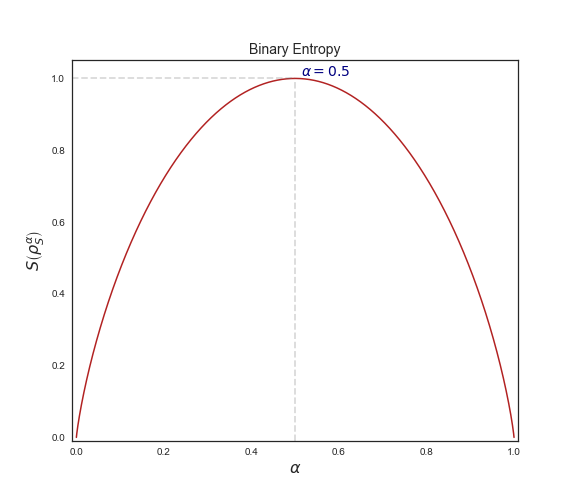
\includegraphics[width=0.6\textwidth]{Figures/Binary_entropy.png}
\caption{Binary Entropy  as a function of binary outcome probability $\alpha$.}
\end{figure}
that is a positive metric function of $\alpha\in [0,1]$, which is 0 for separable global states ($\alpha=0,1$) and reaches its maximum for the maximally entangled Bell state ($\alpha=1/2$). In this latter example the entropy is maximal and it corresponds to a complete ignorance on the subsystem $S$. Observe that the expression given in \eqref{CH1:Binary_entropy} is nothing but the binary entropy function \cite{mackay_information_2003} which is equivalent to the Shannon entropy \cite{shannon_mathematical_1948} of the probability vector $(\alpha,1-\alpha)$.

From the latter example we can see that in general, given a pure state $\ket{\Psi}$ of a composite system $\mathcal{H}=\mathcal{H}_{S}\otimes\mathcal{H}_{E}$ with generic dimensions $d_S = \operatorname{dim}\mathcal{H}_{S}\leq d_E = \operatorname{dim}\mathcal{H}_E$, one gets that
\begin{equation}
0\leq S(\rho_S)\leq \ln d_S.
\label{CH1:inequality_entropy}
\end{equation}
Here $S(\rho_S)= 0$ for separable state, $\ket{\Psi} = \ket{u}\otimes\ket{v}$, while $S(\rho_S)=\ln d_S$ for maximally entangles states,
\begin{equation}
|\Psi\rangle=\frac{1}{\sqrt{d_{S}}} \sum_{k=1}^{d_{S}}\left|u_{k}\right\rangle \otimes\left|v_{k}\right\rangle,
\label{CH1:spearable_state}
\end{equation}
with $\{u_k\}, \{v_k\}$ are the orthogonal basis for each of system and environment.
The von Neumann entropy is a measure of entanglement which leads to an objective lack of knowledge\footnote{In general entropy provides a tool that can be used to quantify entanglement, although other entanglement measures exist \cite{plenio_introduction_2006} If the overall system is pure, the entropy of one subsystem can be used to measure its degree of entanglement with the other subsystems. In particular for bipartite pure states, the von Neumann entropy of reduced states is the unique measure of entanglement in the sense that it is the only function on the family of states that satisfies certain axioms required of an entanglement measure. Being this the reason why we only introduce this entropy.}. In fact, this objective ``lack of knowledge'' is related to the state of the system, because even if we had know everything about the state of the universe,  the state of any system (small portion of the universe) could be mixed \cite{gemmer_distribution_2003,page_average_1993}. This is something astonishing since this lack of knowledge came form nothing but the nature of quantum mechanics, and no randomness was introduced\footnote{Classically the complete knowledge of the state of the universe implies a complete knowledge of the state of any subsystem. Understanding why in the case of classical mechanics, randomness  was artificially add to the description.}.
\newline
Having very clear all these concepts, in the following we will show that thermalisation is a generic property of pure states of the universe, in the sense that for overwhelming majority of them, the reduced state of the system is the canonical mixed state. As a conclusion we can state that the postulate of equal a prior probability, which refers to ensembles or time averages of states of the universe, and as such relies on a subjective lack of information, can be disregard and one can refer only to pure state of the universe. The lack of of information which will give a canonical density matrix for the system is just a physical consequence of entanglement between  the system and its environment.
\subsection{Canonical Typicality}
In this part we would like to show that the principle of equal prior probability, which can not be proved, should be replaced with the principle of \textit{Canonical typicality}, which is based on individual states rather than ensembles or time averages, and most importantly, can be proved.
\newline
Consider a large quantum mechanical system, ``The Universe'', which we decompose in two parts, the system $S$ and the environment $E$\footnote{Here it is implicit that the simension of the environment is much larger than the one of the system.}. Now, suppose the universe has to obey some global constraint $R$, which translates into the choice of a subspace of the total Hilbert space, say
 \begin{equation}
 \mathcal{H}_{R} \subset \mathcal{H}_{S} \otimes \mathcal{H}_{E}
 \label{CH1:Tipicality_1}
 \end{equation}
As we mentioned before, the dimensions of $\mathcal{H}_{S}$, $\mathcal{H}_{E}$  and $\mathcal{H}_{R}$ will be denote by $d_S$, $d_E$ and $d_R$ respectively. In the standard approach to statistical mechanics, as we aforementioned, the restriction is imposed on the total energy. However, as \textit{Popescu et. al.} mention in \cite{popescu_entanglement_2006,popescu_foundations_2005}, this restriction can be let to be completely arbitrary.
\newline
Using the definition of the equiprobable state in \eqref{CH1:equiprobable_state}, we know that $\mathcal{E}_R$ is the maximally mixed state in $\mathcal{H}_R$, in which pure state has equal probability\footnote{As Popescu mention in his paper, this corresponds to the standard intuition in classical mechanics of assigning equal a priori probabilities to all states of the universe consistent with the constraints \cite{popescu_entanglement_2006,popescu_foundations_2005}.}.
\newline
The \textit{canonical state} of the system $S$ is defined as the trace over the environment,
\begin{equation}
\Omega_{S}=\operatorname{Tr}_{E} \mathcal{E}_{R}.
\label{CH1:Canonical_state}
\end{equation}

Instead of considering the universe in the equiprobable state $\mathcal{E}_R$, which describes subjective ignorance, we consider the universe to be in a random pure state $\ket{\phi}\in \mathcal{H}_R$. In such a case the system will be described by the its reduced density matrix
\begin{equation}
\rho_{S}=\operatorname{tr}_{B}(|\phi\rangle\langle\phi|)
\label{CH1:Reduced_density_random_pure_state}
\end{equation}
Here we ask ourselves, how different is $\rho_S$ form the canonical state $\Omega_S$. The answer to this is provided by \textit{Popescu et. al.} in \cite{popescu_entanglement_2006,popescu_foundations_2005}, which states that $\rho_S$ is very close to $\Omega_S$ for every pure state compatible with the constraint $R$.
That is, for almost every pure state of the universe, the system behaves as if the universe were actually in the equiprobable mixed state $\mathcal{E}_R$.
\newline
Nevertheless, it is important to stress that $\Omega_S$ is not necessarily the thermal canonical state \eqref{CH1:equiprobable_canonical_8}, but rather a generalised canonical state with respect to the arbitrary restriction $R$ chosen\footnote{The thermodynamic interpretation is recover is the restriction imposed coincide with the total energy. In that case we can state that  almost every pure state $\ket{\phi}$ of the universe is such that the system $S$ is approximately in the canonical thermal state $e^{-\beta\hat{H}_S}/Z$. }.
\newline
As an illustrative example, we can interpret this result by representing our universe obeying the global constraint $R$ as a map chart in which we see nothing but a vast ocean representing the equiprobable states in $\mathcal{H}_R$ and some islands representing those states who differ drastically from the canonical state. Particularly we represent with a boat a random picked state in the universe, as one can see, for the vast majority of random choices we have, this boat would land in a portion of this ocean.

\begin{figure}[h!]
\centering

\includegraphics[width=0.9\textwidth]{Figures/ocean-of-typicality.png}
\caption{Illustration of the typicality in a map chart. The boat here refers to a random picked state in our universe. Here the islands refer to those states who radically differ from the Canonical state.}
\end{figure}


\subsection{Quantitative Arguments behind Typicality}
In order to formally express these ideas, it is important to explain with more detail the meaning of what we expressed in the latter part. To start with this is is necessary first to define a notion of distance between states $\rho_S$ and $\Omega_S$, as well as a measure over which pure states $\ket{\phi}$ are defined.
\newline
To compute the distance between $\rho_S$ and the canonical state $\Omega_S$ we will use the trace distance, $||\rho_S-\Omega||_1$, which is defined via the trace norm
\begin{equation}
||\rho||_1=\operatorname{Tr}|\rho|=\operatorname{Tr}\left(\sqrt{\rho^{\dagger} \rho}\right)
\label{CH1:Trace_distance}
\end{equation}
This distance basically represents the maximal difference in probability of obtaining any outcome for any measurement performed on the states $\rho_S$ and $\Omega_S$. This can be clearly seen if we write explicitly the definition of an induced norm
\begin{equation}
\|\rho\| = \sup_{\|M\|=1} |\operatorname{Tr}(\rho M)|.
\end{equation}
Using this, we can say that the trace distance measures how difficult is to know $\rho_S$ and $\Omega_S$ via a measurement $M$, explicitly this is
\begin{equation}
\left|\operatorname{Tr}\left(\rho_{S} M\right)-\operatorname{Tr}\left(\Omega_{S} M\right)\right| \leq\left\|\rho_{S}-\Omega_{S}\right\|_{1}\|M\|,
\label{CH1:inequality1_tipicality}
\end{equation}
An important fact to stress is choice of this distance, one could wonder, why do not we use other operator distance such like Hilbert-Schmidt norm, which is defined by taking the root square of the trace, instead of the trace of the root square, as the trace norm is defined. The reason to do this is simply because the Hilbert-Schmidt distance in higher dimensions can tend to be very small even when the states have a disjoint support\cite{facchi_quantum_2017}. To explain this in more clearly, consider in $\mathbb{C}^{2d}$ the two states $\rho_1 = \mathbb{I}_1/d$ and $\rho_2 =(1-\mathbb{I}_1)/d$, where $\mathbb{I}_1$ is a projector over $d$ dimensions. An important fact over these states is that they have disjoint supports just as we mentioned before. So computing the distance between these two states give us
\begin{equation}
\left\|\rho_{1}-\rho_{2}\right\|_{1}=2, \quad\left\|\rho_{1}-\rho_{2}\right\|_{2}=\sqrt{\frac{2}{d}},
\label{CH1:Example_1}
\end{equation}
and then the trace norm give us a constant while the Hilbert-Schmidt distance decreases d increases $1/\sqrt{d}$.
\newline
Consider $\ket{\phi}$ to be a pure state in $\mathcal{H}_R$, with respective dimension $d_R$. As the state is normalized ($\langle\phi | \phi\rangle=1$) this immediately tells us  that the pure state $\ket{\phi}$ belongs to a real sphere ($2d_R-1$)-dimensional. Therefore, the states we are interested in live over the surface of a sphere of $d_R$ dimensions, thus to random samle one of this states we will have to sample with the measure $\sigma(\mathbb{S}^{2d_R-1})$, which is known as the Haar measure. From this definition, it is clear to see if the selected random state over the Haar measure, the average state of the universe in $\mathcal{H}_R$ is nothing but the equiprobable state, and then we get that average state of the system is nothing but the canonical state $\Omega_S = \langle \rho_S\rangle$.
\newline
Now with the notion of the distance we chose to work with, and the space where these pure states live in, we are ready to announce the general result in typicality.
\newline
\textbf{Theorem of Canonical Typicality \cite{popescu_entanglement_2006,popescu_foundations_2005}}.
\newline
\textit{For a random chosen state, sampled with the Haar measure, $\ket{\phi}\in\mathcal{H}_R\subset\mathcal{H}_S\otimes\mathcal{H}_B$ and arbitrary $\varepsilon >0$ the distance between the reduced density matrix $\rho_{S}=\operatorname{Tr}_{E}(|\phi\rangle\langle\phi|)$ and the canonical state $\Omega_S=\operatorname{Tr}_E\mathcal{E}_R$ is given probabilistically by:}
\begin{equation}
\operatorname{Prob}\left(\left\|\rho_{S}-\Omega_{S}\right\|_{1} \geq \eta\right) \leq \eta^{\prime},
\label{CH1:Typicality_result_1}
\end{equation}

\textit{where}
\begin{equation}
\eta=\varepsilon+\sqrt{\frac{d_{S}}{d_{E}^{\mathrm{eff}}}}, \quad \eta^{\prime}=2 \exp \left(-C d_{R} \varepsilon^{2}\right),
\label{CH1:Typicality_result_1_1}
\end{equation}
\textit{with}

\begin{equation}
C=\frac{1}{18 \pi^{3}}, \quad d_{E}^{\mathrm{eff}}=\frac{1}{\operatorname{Tr} \Omega_{E}^{2}}\geq \frac{d_R}{d_S}, \quad \Omega_{E}=\operatorname{Tr}_{S} \mathcal{E}_{R}
\label{CH1:Typicality_result_1_2}
\end{equation}
Form the latter result we notice that $\eta$ and $\eta'$ are small quantities, and then, the state will be close to the canonical state with high probability, whenever $d^{\mathrm{eff}}_E\ggg d_S$ and $d_R\varepsilon^2\ggg 1 \ggg \varepsilon$. The latter condition can be ensured when $d_R\ggg 1$.
\newline
So what our latter results holds is that probabilistically speaking if the dimension of the accessible space ($d_R$) is large enough, we will have that for the overwhelming majority of choices of random pure states, we will have always (almost) that every system, with small enough dimension, will be indistinguishable from the canonical state. Even more, \textit{Popescu et. al.} get an expression to show how the fluctuations around the average behave. For this they get the next result
\newline
\begin{equation}
\left\langle\left\|\rho_{S}-\Omega_{S}\right\|_{1}\right\rangle \leq \sqrt{\frac{d_S}{d_E^{\mathrm{eff}}}}\leq\sqrt{\frac{d_{S}^{2}}{d_{R}}},
\label{CH1:Typicality_result_2}
\end{equation}
which tells us if the dimension of our accessible space $d_R$ is large enough, compared to the dimension of the system, the fluctuations on the system are also very small. Thus these two results give us the quantitative arguments of typicality.
\newline
Up to this moment we have provided the qualitative as well quantitative arguments to show why typicality gives us an approach different than the equal a priori probability, that can not be proved, and replace it with a key quantum property, entanglement, which provides us a subjective lack of knowledge and more important that can be proved, to show that thermalisation turns up to be a generic property of pure states of the universe. However, despite this result explains very well the reason why by choosing randomly a state $\ket{\phi}$ over the Haar measure, it coincides with the canonical state in almost all cases, it does not explain the way a state out of equilibrium (atypical state) under certain unitary evolution can reach its thermalisation. This means that the latter result is Kinematic rather than dynamical and therefore can not be used to explain how a thermalisation in a system can occur. The goal of the next section is to introduce a work done by \textit{Linden et. al.} \cite{linden_quantum_2009} in which a dynamical approach is done in order to explain how thermalisation can occur in a system reliant on a given unitary dynamic.

\section{Evolution Towards Equilibrium.}
As we above-mentioned, the latter result is only valid for a given time and state, meaning that this can not be used to study the how thermalisation occurs. Now we are interested in states that are atypical, in the sense that are going to be those states such that drastically differ from the canonical state. Even though, we might think that if typicality holds, most evolutions will quickly drive us from a state in which the system is not thermalised into one that is, and that system will remain in this states of ``thermalisation'' for most of its evolution. Nevertheless, there are some problems which are worth to mention about why this is much harder problem to solve. In the following we will show what could be named as the roadmap of what is needed to be proved in order to show that a thermal state has thermalised.
\begin{itemize}
\item \textbf{Equilibration}: It is possible to affirm that a system will equilibrate if its states evolve towards a particular state, which can be in the more general case a mixed state, and remains in that state, or at least quite close to it, for every time\footnote{Even though this definition does not specify the sort of equilibrium state of the system, the state of equilibrium will strongly depend on the initial condition of the system as well as the initial conditions over its environment. }
\item \textbf{Environment state independence}: The equilibrium state that the system reaches has to be independent of the initial state of the environment, this is, when the system reaches its state of equilibrium, this state should depend only on macroscopic parameters of the environment, like temperature or similar macroscopic parameters.
\item \textbf{System state independence}: If the system is much smaller than the environment, the state of equilibrium should not depend of its initial state.
\end{itemize}
Having this in mind, it is possible to tackle these problems one by one. An interesting result is provided by \textit{Linden et. al.}  \cite{linden_quantum_2009}, where they manage to prove that with relatively full generality, equilibrium is an universal property of Quantum systems and even more that equilibrium state does not depend on the state of the environment.
\newline
To completely understand \textit{Linden et. al.} work is necessary to first understand couple of definitions they provide in their paper  \cite{linden_quantum_2009}.
\newline
\textbf{Universe:} Here we will refer always to a large quantum universe living in a Hilbert space $\mathcal{H}$. As previously, we are considering an universe that can be decomposed in two, in this decomposition we refer the system $S$ to a small part of the Hilbert space and the rest we will call it the environment. Explicitly we decompose the Hilbert space of the universe as a tensor product of the Hilbert space of the system and the environment, $\mathcal{H}=\mathcal{H}_S\otimes \mathcal{H}_E$, where $d_S$ and $d_E$ the respective dimension of the system and the environment. Notice that here the environment nor the system have provided with any special property. Here the system could be a single particle or even a section of a lattice.
\newline
\textbf{Hamiltonian:} The evolution of the universe will be governed by a Hamiltonian given by
\begin{equation}
\hat{H}=\sum_{k}E_k\ket{E_k}\bra{E_k}.
\label{CH1:Hamiltonian_universe_linden}
\end{equation}
with $\ket{E_k}$ the eigenstate in the energy basis with energy $E_k$. The main assumption here is related with the possible values of energies this Hamiltonian can have. The only requirement needed the Hamiltonian to have non-degenerate energy gaps.
\newline
It is said that a Hamiltonian has no-degenerate energy gaps if any non-zero difference of eigenvalues of energy determine the two energy values involved. That is, for any four eigenstates with energy $E_k$, $E_\ell$, $E_m$, $E_n$, satisfy that if $E_{k}-E_{\ell}=E_{m}-E_{n}$, then $m=n$ and $k=\ell$, or $k=m$ and $\ell = n$. Which turns out to be the same condition of imposing that the energy levels have to be non-degenerate.\newline
Notice that the restriction imposed to the Hamiltonian is a extremely natural constraint, this is because all Hamiltonian that lack of symmetries have non-degenerate energies, so we refer to a set of Hamiltonians with measure $1$.
\newline
\textbf{Notation:} We will work here with pure states for the universe represented by $\ket{\Psi(t)}$ with a density matrix state given by $\rho(r) =\ket{\Psi(t)}\bra{\Psi(t)}$. As above-mentioned, the state of the system is obtained by tracing out the environment at a time $t$, that is, $\rho_S(t)=\operatorname{Tr}_E \rho(t)$. Similarly we define the state of the environment as $\rho_E(t)=\operatorname{Tr}_S \rho(t)$.\newline
We define a convenient quantity which is the transient state, or the time averaged state $\omega$
\begin{equation}
\omega=\langle\rho(t)\rangle_{t}=\lim _{\tau \rightarrow \infty} \frac{1}{\tau} \int_{0}^{\tau} \rho(t) d t,
\label{CH1:average_time_state}
\end{equation}
and similarly we define $\omega_s$ and $\omega_E$ as the time averaged state of the system and the environment respectively.\newline
It is also convenient to re introduce a concept we have already used, the effective dimension of a mixed state $\rho$:
\begin{equation}
d^{\mathrm{eff}}(\rho)=\frac{1}{\operatorname{Tr}\left(\rho^{2}\right)},
\label{CH1:Effective_dimension}
\end{equation}
which is generally a better measurement of the effective dimension than the dimension of the support of $\rho$. This measure roughly tells us how many states contribute to the mixture\footnote{Particularly, a mixture of $n$ orthogonal states with equal probability has effective dimension of $n$ }, carrying the probabilistic weight of different states in the mixture, and is a continuous measure.
\newline
With the concepts aforementioned Linden et. al. \cite{linden_quantum_2009} are able to mathematically prove
\begin{quote}
\textit{Every pure state of a quantum universe, composed by a large number of eigenstates of energy\footnote{The reason why we need the global state to have many eigenstates of energy is because by imposing this we can assure that there will be a large quantity of changes throughout the evolution of the system.} such that evolves under an arbitrary Hamiltonian, is such that every system small enough will equilibrate.}
\end{quote}
The reason why the latter statement requires the universe to have many changes in its time evolution, is because for equilibration to take place it is needed that part of the information of the initial state of the system leaves the system and enters in the environment. This notion of evolving through many states can be mathematically encapsulated via the effective dimension of the time average state $\omega=\langle\rho(t)\rangle_{t}$, and the connection between this and the number of eigenstates is with ease seen by expanding $\ket{Psi(t)}$ as
\begin{equation}
|\Psi(t)\rangle=\sum_{k} c_{k} e^{-i E_{k} t}\left|E_{k}\right\rangle
\label{CH1:expansion_1}
\end{equation}
where $\sum_{k}\left|c_{k}\right|^{2}=1$ and hence
\begin{equation}
\rho(t)=\sum_{k, l} c_{k} c_{l}^{*} e^{-i\left(E_{k}-E_{l}\right) t}\left|E_{k}\right\rangle\left\langle E_{l}\right|,
\label{CH1:expansion_2}
\end{equation}
which can be expanded and written as
\begin{equation}
\begin{aligned}
\rho(t)=\underbrace{\sum_{n}\|c_{n}\|^{2}\ket{E_{n}}\bra{E_{n}}}_{\omega}&+\underbrace{\sum_{m \neq n} c_{n} c_{m}^{*}\ket{E_{n}}\bra{E_{m}} e^{-i t\left(E_{n}-E_{m}\right)}}_{\lambda (t)} \\
&=\omega+\lambda(t),
\end{aligned}
\label{CH1:Expansion_to_use_after}
\end{equation}
Now in the case of non-degeneracy of the energy levels we have
\begin{equation}
\omega=\langle\rho(t)\rangle_{t}=\sum_{k}\left|c_{k}\right|^{2}\left|E_{k}\right\rangle\left\langle E_{k}\right|,
\label{CH1:expansion_3}
\end{equation}
leading us to 
\begin{equation}
d^{\mathrm{eff}}(\omega)=\frac{1}{\operatorname{Tr}\left(\omega^{2}\right)}=\frac{1}{\sum_{k}\left|c_{k}\right|^{4}}.
\label{CH1:expansion_4}
\end{equation}
Thus formally the statement above-mentioned can be mathematically written in terms of central quantity $D\left[\rho_{S}(t), \omega_{S}\right]$\footnote{Here has in the case of typicality we use the trace distance.}, the distance between $\rho_S(t)$, the state of the system at a time $t$, and its time average, $\omega_{S}=\left\langle\rho_{S}(t)\right\rangle_{t}$. The difference between $\rho_S(t)$ and $\omega_{S}$ in the energy eigenstates can be written as
\begin{equation}
\rho_{S}(t)-\omega_{S}=\sum_{m \neq n} c_{m} c_{n}^{*} e^{-i\left(E_{m}-E_{n}\right) t} \operatorname{Tr}_{E}\left|E_{m}\right\rangle\left\langle E_{n}\right|.
\label{CH1:expansion_5}
\end{equation}
Since in general we know that $\rho_S(t)$ fluctuates around the state $\omega_S$, it is evident that the distance between them will change over time. Therefore, in order to characterise these fluctuations we will be interested in the time average of distance $\langle D\left[\rho_{S}(t), \omega_{S}\right]\rangle_t$, so the value this average takes will tell us about where the system is spending most of its time. In other words $\langle D\left[\rho_{S}(t), \omega_{S}\right]\rangle_t$ will be small when the system equilibrates to $\omega_S$.\newline
To be able to prove what is announced as the \textit{Theorem 1} in \cite{linden_quantum_2009}
it is useful to relate the trace distance to the square of the Hilbert-Schmidt distance using a standard bound provided in \cite{fuchs_cryptographic_1999}
\begin{equation}
D\left(\rho_{1}, \rho_{2}\right)=\frac{1}{2} \operatorname{Tr}_{S} \sqrt{\left(\rho_{1}-\rho_{2}\right)^{2}} \leq \frac{1}{2} \sqrt{d_{S} \operatorname{Tr}_{S}\left(\rho_{1}-\rho_{2}\right)^{2}}.
\label{CH1:Linden_proof_1}
\end{equation}
By using the concavity of the square-root function, we therefore have
\begin{equation}
\left\langle D\left[\rho_{S}(t), \omega_{S}\right]\right\rangle_{t} \leq \sqrt{d_{S}\left\langle\operatorname{Tr}_{S}\left[\rho_{S}(t)-\omega_{S}\right]^{2}\right\rangle_{t}},
\label{CH1:Linden_proof_2}
\end{equation}
which will provide us the bound we need to proof the theorem. Now using \eqref{CH1:expansion_5} we write
\begin{equation}
\left\langle\operatorname{Tr}_{\mathcal{S}}\left[\rho_{\mathcal{S}}(t)-\omega_{\mathcal{S}}\right]^{2}\right\rangle_{t}=\sum_{m \neq n} \sum_{k \neq l} \mathcal{T}_{k l m n} \operatorname{Tr}_{\mathcal{S}}\left(\operatorname{Tr}_{E}\left|E_{k}\right\rangle\left\langle E_{l}\left|\operatorname{Tr}_{E}\right| E_{m}\right\rangle\left\langle E_{n}\right|\right),
\end{equation}
where $\mathcal{T}_{k l m n}=c_{k} c_{l}^{*} c_{m} c_{n}^{*} e^{-i\left(E_{k}-E_{l}+E_{m}-E_{n}\right) t}$. Computing this time average taking into account that the Hamiltonian has non-degenerate energy gaps\footnote{This condition is reflected in the evaluation by considering the terms where $k\neq\ell$ and $m\neq n$, leading to $m=\ell$ and $k=n$ are the only terms that contribute.} we find  that

\begin{equation}
\begin{aligned}
\left\langle\operatorname{Tr}_{S}\left[\rho_{S}(t)-\omega_{S}\right]^{2}\right\rangle_{t} &=\sum_{k \neq l}\left|c_{k}\right|^{2}\left|c_{l}\right|^{2} \operatorname{Tr}_{S}\left(\operatorname{Tr}_{E}\left|E_{k}\right\rangle\left\langle E_{l}\left|\operatorname{Tr}_{E}\right| E_{l}\right\rangle\left\langle E_{k}\right|\right) \\
&=\sum_{k \neq l}\left|c_{k}\right|^{2}\left|c_{l}\right|^{2} \sum_{s s^{\prime} b b^{\prime}}\left\langle s b | E_{k}\right\rangle\left\langle E_{l} | s^{\prime} b\right\rangle\left\langle s^{\prime} b^{\prime} | E_{l}\right\rangle\left\langle E_{k} | s b^{\prime}\right\rangle\\
&=\sum_{k \neq l}\left|c_{k}\right|^{2}\left|c_{l}\right|^{2} \sum_{s s^{\prime} b b^{\prime}}\left\langle s b | E_{k}\right\rangle\left\langle E_{k} | s b^{\prime}\right\rangle\left\langle s^{\prime} b^{\prime} | E_{l}\right\rangle\left\langle E_{l} | s^{\prime} b\right\rangle \\
&=\sum_{k \neq l}\left|c_{k}\right|^{2}\left|c_{l}\right|^{2} \operatorname{Tr}_{E}\left(\operatorname{Tr}_{S}\left|E_{k}\right\rangle\left\langle E_{k}\left|\operatorname{Tr}_{S}\right| E_{l}\right\rangle\left\langle E_{l}\right|\right)\\
&=\sum_{k \neq l} \operatorname{Tr}_{E}\left[\operatorname{Tr}_{S}\left(\left|c_{k}\right|^{2}\left|E_{k}\right\rangle\left\langle E_{k}\right|\right) \operatorname{Tr}_{S}\left(\left|c_{l}\right|^{2}\left|E_{l}\right\rangle\left\langle E_{l}\right|\right)\right] \\
&=\operatorname{Tr}_{E} \omega_{E}^{2}-\sum_{k}\left|c_{k}\right|^{4} \operatorname{Tr}_{S}\left[\left(\operatorname{Tr}_{E}\left|E_{k}\right\rangle\left\langle E_{k}\right|\right)^{2}\right] \\
&\leq \operatorname{Tr}_{E} \omega_{E}^{2},
\end{aligned}
\label{CH1:Linden_proof_3}
\end{equation}
where $\omega_E=\operatorname{Tr}_S \omega$. To obtain a further bound, we invoke weak
sub-additivity of the Re\'enyi entropy \cite{camilo_strong_2019}
\begin{equation}
\operatorname{Tr}\left(\omega^{2}\right) \geq \frac{\operatorname{Tr}_{E}\left(\omega_{E}^{2}\right)}{\operatorname{rank}\left(\rho_{S}\right)} \geq \frac{\operatorname{Tr}_{E}\left(\omega_{E}^{2}\right)}{d_{S}},
\label{CH1:Linden_proof_4}
\end{equation}

and therefore combining \eqref{CH1:Linden_proof_2}, \eqref{CH1:Linden_proof_3} and \eqref{CH1:Linden_proof_4} we get
\begin{equation}
\left\langle D\left[\rho_{S}(t), \omega_{S}\right]\right\rangle_{t} \leq \frac{1}{2} \sqrt{d_{S} \operatorname{Tr}_{E}\left(\omega_{E}^{2}\right)} \leq \frac{1}{2} \sqrt{d_{S}^{2} \operatorname{Tr}\left(\omega^{2}\right)},
\label{CH1:Inequality_last}
\end{equation}

which by taking the definition of effective dimension, we get the main result shown in \cite{linden_quantum_2009}
\begin{equation}
\left\langle D\left[\rho_{S}(t), \omega_{S}\right]\right\rangle_{t} \leq \frac{1}{2} \sqrt{\frac{d_{S}}{d^{\mathrm{eff}}\left(\omega_{E}\right)}} \leq \frac{1}{2} \sqrt{\frac{d_{S}^{2}}{d^{\mathrm{eff}}(\omega) }}.
\label{CH1:Result_linden}
\end{equation}
As we can see the result obtained by Linden et. al. tell us that the vast majority of quantum systems which the dynamic of the universe is governed by a Hamiltonian with no gaps, will spend most of its time close to its equilibrium state independently of its initial state\footnote{Notice that the last result is not necessarily considering that the state of equilibration will coincide with the canonical state, this result is very general. Exponential bounds can be achieve if we consider the energy eigenvalues of the Hamiltonian to have no rational dependencies, this restriction leads to exponential bound in $d^{\mathrm{eff}}(\omega)$ (check Appendix C in \cite{linden_quantum_2009}) . }.\\
To illustrate this result we will picture an universe as the one described before in which the islands refer to the systems regions of the universe such that are atypical and the ocean the region which represent the region where the system equilibrates. As shown in the figure 
\ref{Island_of_equilibrium} we can start from a region in the island (out of the equilibrium) and going out to the ocean (region of equilibrium), as is shown we jump from the island to the ocean so that in average we spend most of the time out of the island.
\begin{figure}[h!]
\centering
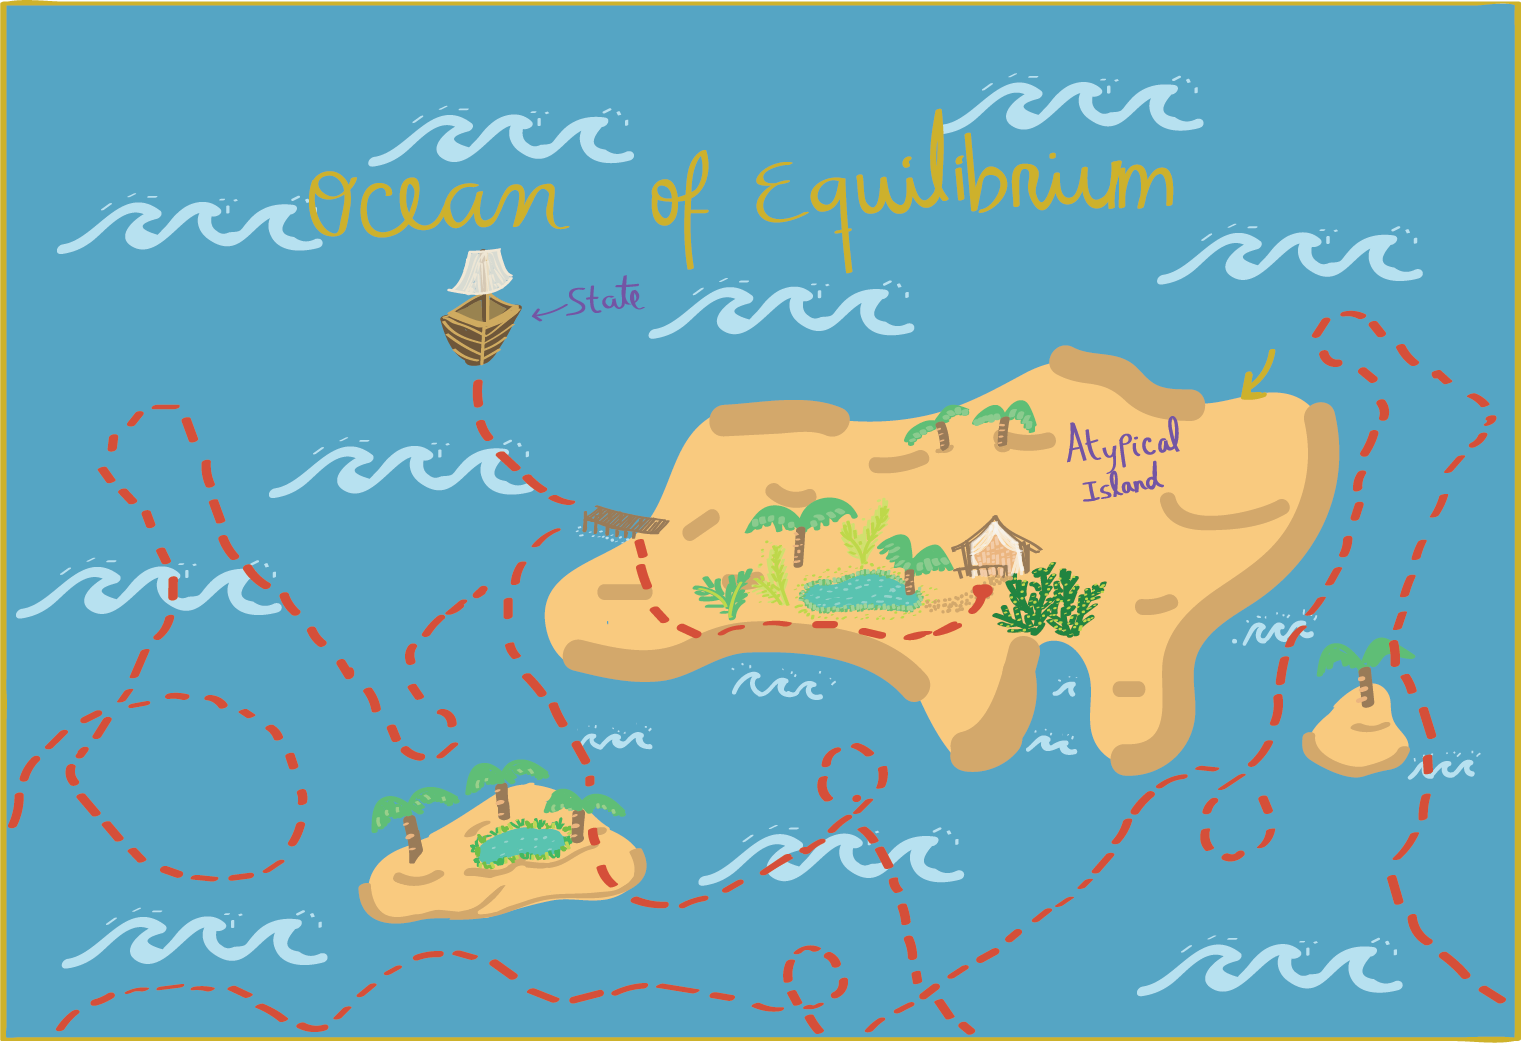
\includegraphics[width=0.9\textwidth]{Figures/ocean-of-equilibrium.png}
\caption{Illustration of the result from Linden et. al. drawn in a map chart. The ship here refers to the state sailing in our universe. Whereas the islands refer to the region in which our ship is out of equilibrium.}
\label{Island_of_equilibrium}
\end{figure}
Even though, this results tell us that apparently the quantum property of systems is to be close to its equilibrium state, it does not take into consideration how fast it is getting to this state. Since the time averages are taken, we can say that the term of $\lambda$ goes to zero in trace norm, that is $\langle\| \lambda\|_1\rangle_t \to 0$, this can be assured since the \textit{Random phase postulate} described above, holds. However, it is easy to see that if we take a state which  its energy eigenvalues are very close to each others, the time it will take to equilibrate is exponentially large. It is not of our purpose to measure how fast a system presenting but instead we present an alternative to the \textit{Random phase postulate} in which we present an alternative form for the special case in which the energy eigenvalues are very close to each other.\newline
To better explain our idea consider an universe $\ket{\Psi}$ which is decomposed on two states that are very close to each other, for example a state of the universe belonging to an shell of a defined energy, the energy eigenstates $\ket{E_n}$ and $\ket{E_m}$, the state of the universe can be written as
\begin{equation}
\begin{aligned}
\rho &= \ket{\Psi}\bra{\Psi}\\
&= \|c_n\|^2 \ket{E_n}\bra{E_n} +  \|c_m\|^2 \ket{E_m}\bra{E_m} \\
& + c_n c^{*}_m  \ket{E_n}\bra{E_m}+ c_m c^{*}_n \ket{E_m}\bra{E_n},
\end{aligned}
\label{CH1:State_as_function_of_time}
\end{equation}
if we take the partial trace of the equation \eqref{CH1:State_as_function_of_time} this will lead us to the state of the system,
\begin{equation}
\begin{aligned}
\rho_S &= \operatorname{Tr}_E \rho = \operatorname{Tr}_E  \ket{\Psi}\bra{\Psi}\\
&= \|c_n\|^2\operatorname{Tr}_E  \ket{E_n}\bra{E_n} +  \|c_m\|^2 \operatorname{Tr}_E \ket{E_m}\bra{E_m} \\
& + c_n c^{*}_m  \operatorname{Tr}_E \ket{E_n}\bra{E_m} + c_m c^{*}_n \operatorname{Tr}_E \ket{E_m}\bra{E_n}.
\end{aligned}
\label{CH1:State_as_function_of_time_system}
\end{equation}
Something we notice from \eqref{CH1:State_as_function_of_time_system} is that since we consider the state to have its eigenvalues of energy to be quite close to each other, by using typicality we get that $\operatorname{Tr}_E \ket{E_n}\bra{E_n} =\operatorname{Tr}_E \ket{E_m}\bra{E_m} = \Omega(E)$, with $\Omega(E)$ the canonical state. Therefore the equation \eqref{CH1:State_as_function_of_time_system} can be written as
\begin{equation}
\rho_S= \Omega(E) + c_n c^{*}_m  \operatorname{Tr}_E \ket{E_n}\bra{E_m} + c_m c^{*}_n \operatorname{Tr}_E \ket{E_m}\bra{E_n}.
\label{CH1:State_as_function_of_time_system_typicality}
\end{equation}
As we did not consider any evolution time from the result of typicality we realise that the two last terms in equation \eqref{CH1:State_as_function_of_time_system_typicality} should cancel in order to be consistent with the result of typicality discussed before. The only way those terms vanish is by a property that we will call ultra-orthogonality, which refers to an apparent orthogonality of states with respect to the partial trace, that it
\begin{equation}
\operatorname{Tr}_E \ket{E_n}\bra{E_m} = \operatorname{Tr}_E \ket{E_m}\bra{E_n} = 0
\end{equation}
In consideration of that, we state that the mechanism which makes the systems to equilibrate emerge as a consequence of typicality and is encapsulated in what we name by ultra-orthogonality under partial trace. thus in equation \eqref{CH1:expansion_5} we see that this difference will be immediately zero, independently of the time average, in the case we consider typical states (thermal states).
\newline
From these ideas we decided to explore this super-orthogonality in a physical system such that can be solved analytically (or numerically), this to have complete knowledge of the state of our universe, to then take a small portion of it. Thus in order to do that, it is necessary to be able to compute with relative easiness the diagonalization of our universe as well as the reduced states of it in an efficient way\footnote{We emphasise that it has to be efficient because the trend of the Hilbert space is to grow exponentially with its dimension, so we want to be able to handle large dimensions in the Hilbert space as well as compute them on a computer. }. In the following sections we will provide the background required to understand the choice of the system we made as well as detailed calculations which provide a full characterization of this system and its reduced states. 